%-----------------------------------------------------------------------------
%
%               Template for sigplanconf LaTeX Class
%
% Name:         sigplanconf-template.tex
%
% Purpose:      A template for sigplanconf.cls, which is a LaTeX 2e class
%               file for SIGPLAN conference proceedings.
%
% Guide:        Refer to "Author's Guide to the ACM SIGPLAN Class,"
%               sigplanconf-guide.pdf
%
% Author:       Paul C. Anagnostopoulos
%               Windfall Software
%               978 371-2316
%               paul@windfall.com
%
% Created:      15 February 2005
%
%-----------------------------------------------------------------------------


\documentclass{sigplanconf}

% The following \documentclass options may be useful:

% preprint      % Remove this option only once the paper is in final form.
% 10pt          To set in 10-point type instead of 9-point.
% 11pt          To set in 11-point type instead of 9-point.
% authoryear    To obtain author/year citation style instead of numeric.

\usepackage{amsmath}
\usepackage{natbib}
\usepackage{graphicx}
\usepackage{wrapfig}
\usepackage{caption}
\usepackage{url}


\begin{document}

\special{papersize=8.5in,11in}
\setlength{\pdfpageheight}{\paperheight}
\setlength{\pdfpagewidth}{\paperwidth}

\conferenceinfo{CONF 'yy}{Month d--d, 20yy, City, ST, Country} 
\copyrightyear{20yy} 
\copyrightdata{978-1-nnnn-nnnn-n/yy/mm} 
\doi{nnnnnnn.nnnnnnn}

% Uncomment one of the following two, if you are not going for the 
% traditional copyright transfer agreement.

%\exclusivelicense                % ACM gets exclusive license to publish, 
                                  % you retain copyright

\permissiontopublish             % ACM gets nonexclusive license to publish
                                  % (paid open-access papers, 
                                  % short abstracts)

\titlebanner{banner above paper title}        % These are ignored unless
\preprintfooter{short description of paper}   % 'preprint' option specified.

\newcommand{\pname}{KinEdit}

\title{\pname{}: A Tool to Help Developers Refactor Manually}
% \subtitle{View and edit all contexts referring to a common identifier}

\authorinfo{Josh Terrell}
           {California Polytechnic University, San Luis Obispo}
           {jmterrel@calpoly.edu}
% \authorinfo{Name2\and Name3}
%            {Affiliation2/3}
%            {Email2/3}

\maketitle

\begin{abstract}
Some developers do not trust automated refactoring tools to refactor correctly.
Without using refactoring tools, refactoring can take longer and result
in more bugs. Developers do not have to trust automated refactoring tools to
take advantage of some productive features that refactoring tools offer.
Using \pname{}, developers can refactor more quickly, with higher
quality, and without needing to trust automated refactoring tools.
% problem. why propblem is problem. startling sentence (make claim). implication.
\end{abstract}

\category{not sure what to put here..CR-number}{subcategory}{third-level}

% general terms are not compulsory anymore, 
% you may leave them out
% \terms
% term1, term2

\keywords
refactoring, tool, trust

%TODO can work in conjunction with existing tools

\section{Problem and Motivation}
Refactoring is the process of changing the structure of code without changing
its behavior, a process that can improve maintainability~\cite{maintainability}.
Refactoring tools are available for many languages to automate the process of
refactoring. When developers perform a refactoring that a tool can automate for
them, research suggests that they choose to refactor manually 90\% of the
time~\cite{how-refactor}. One of the reasons developers choose to refactor
manually rather than use a tool is because they do not trust that the change
the tool will make will be as they expect~\cite{how-refactor, say-refactor}. 
% NOTE: maybe get rid of details on trust
Some worry that refactoring tools may introduce bugs; others
are concerned with the readability and design of the code produced by the
tools~\cite{say-refactor}.

When manually refactoring, some developers
\textit{lean on the compiler}~\cite{legacy-code, how-refactor}.
For example, when renaming a method, developers may temporarily comment
out the method, resulting
in an error at each call site. The developers can then
use these errors as an aid to navigate quickly between the call sites.
Navigating to the call sites can serve two purposes: to look at the calling
contexts to determine a better name, and to edit each call site to specify
the new method name.

I acknowledge that leaning on the compiler is a common and continuing practice
among software developers. Rather than insisting that they use a refactoring
tool, this paper contributes a new tool
called \pname{} that allows developers to continue to refactor
manually, but supports them with navigation assistance.

\section{Background and Related Work}
There are other tools which also help developers refactor manually. Two of them
are
BeneFactor~\cite{bene-factor} and WitchDoctor~\cite{witch-doctor},
which allow developers to start a refactoring manually and then
complete it automatically.
In contrast, \pname{} allows the developers to refactor completely manually.
% TODO: trust is not addressed by these tools.

GhostFactor takes a different apporach. GhostFactor automatically detects
when a developer has completed a manual refactoring and validates
that the developer has refactored correctly~\cite{ghost-factor}.
In contrast, \pname{} does not help developers with the correctness of
their refactorings, but instead helps them navigate during refactoring.

\section{Approach and Uniqueness}
\pname{} is aimed at supporting the \textit{lean on the compiler} technique
by making it easy for a developer to navigate between related errors introduced
during a refactoring. \pname{} achieves this by opening every related error
in its own editor displayed adjacent in one tab.

Consider the example in the introduction where the developer
wishes to rename a method by first commenting out
the method to find all of the references to it.
On one of the introduced errors, the developer invokes \pname{} by choosing
the ``Show with other Errors...'' option of Eclipse's Quick Fix
menu (Figure~\ref{quick}).

\begin{figure}[h]
\begin{center}
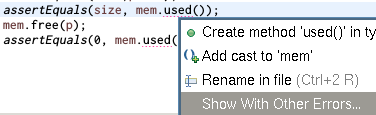
\includegraphics[width=0.35\textwidth]{quick-fix.png}
\caption{Click ``Show with other Errors...'' on an error.\label{quick}}
\end{center}
\end{figure}

After clicking the Quick Fix, \pname{} opens the tab containing one editor
per error as shown in Figure~\ref{mult}. The tab currently shows three
errors in three sub-editors; by using the right-most scrollbar the developer
can view the other nineteen errors introduced by this manual refactoring.
These adjacent editors are designed to facilitate two manual refactoring tasks.
First the developer can view the context of each method reference to enable
her to choose a more appropriate name. Second the developer can use
the editors to rename each call site.

In contrast, without \pname{}, the developer had to
manually determine which error messages were relevant to the refactoring, and
then navigate to each error manually. This process had to be done once for
choosing a name and a second time for making the change. \pname{} makes this
process
easier by automatically collecting all error messages that were introduced by
the manual refactoring, then showing the errors adjacent to one another in a
single tab.

\begin{figure}
\begin{center}
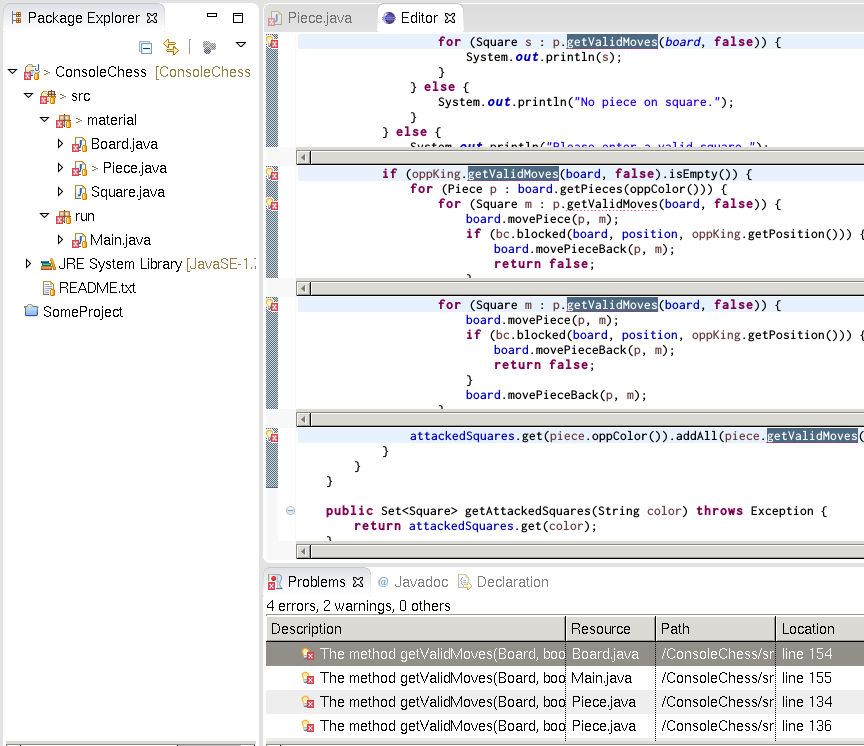
\includegraphics[width=0.50\textwidth]{multiple-editors.png}
\caption{Related errors are each opened in their own editor.\label{mult}}
\end{center}
\end{figure}

This example shows how \pname{} can be used to accomplish a rename refactoring.
\pname{} can also help with other common refactorings.
To name a few, it can assist developers in performing the refactorings
\textit{pull up method}, \textit{push down method}, \textit{add parameter},
\textit{change return type}, and \textit{extract interface}
while enabling the developer to continue refactoring manually. In general,
\pname{} helps with change tasks where a developer must view or edit multiple
references to a particular program element such as a method, variable, or
class.
I implemented \pname{} in Eclipse, and it is freely available on
github at \url{http://todo.com}.

\section{Results and Contributions}
I asked four volunteers to perform two renamings. I asked the volunteers to
determine a better
name for two identifiers, and then rename the identifiers and all references.
One of the tasks was to rename a method used in
ten files. The other was to rename a private instance variable. Two volunteers
were asked to use \pname{} to rename the method, the other were asked
to rename the variable using \pname{}.
For the non-tool renaming task, the volunteers were instructed to rename however
they'd like but without using Eclipse's built-in rename refactor.

The volunteers were confused when \pname{} displayed multiple editors for errors
located only a few lines apart from each other. One possible solution is to
display all references which occur no more than some threshold of lines from
each other together in one editor. Another is to display all errors from one
file in the same editor, but use code folding to fold away the code inbetween.

A volunteer commented that it was difficult to use the tool to perform
a refactoring without a sense of progress. There may be tens of editors
open but the volunteer doesn't know which ones he's viewed or edited.
To help the user, \pname{} might display
some sort of progress indicators to allow the user to know which editors
she has visited, edited, and never visited. Color indicators or a progress
meter at the top may prove to be helpful.

\section{Future Work}
Currently \pname{} has limited functionality, however it has potential to expand
into a more productive tool. \pname{} currently encompasses one primary
feature---opening a window containing each of a given error's related errors
(including iteself). In the future the tool should have some additional
capabilities:

\begin{itemize}
  \item Right click an identifier to open all references to the method, class,
      or variable in the multiple editor window.
  \item In Eclipse's find all references, include a button on the interface
      to open the multiple-editor window.
  \item Provide a listing in Eclipse's Quick Assist (Ctrl+2).
\end{itemize}

\appendix
% \section{Appendix Title}
% 
% This is the text of the appendix, if you need one.

\acks
Thank you Dr. Emerson Murphy-Hill for your guidance through writing this
paper during my summer research internship at North Carolina State University.
I am also very appreciative of the National Science Foundation which made this
research opportunity and many like it possible.

% We recommend abbrvnat bibliography style.

\bibliographystyle{abbrvnat}

% The bibliography should be embedded for final submission.

\softraggedright
\bibliography{error-view}

\end{document}
